
\chapter{Background \& Objectives}

\section{Background}

This project aims to build a website to make it easier and more efficient for beginner SQL learners to create a database that follows database design principles. Database tables are also hard to visualise as well as understand the relationships between them, this project aims at making this process easier. The tool spots trivial mistakes like a table missing a primary key or tables not all being linked by foreign key constraints. It also validates the SQL that the user uploads and informs them of any syntax errors that have been detected.

The main application of this project is to aid students in designing databases. Its aim is to find any errors or possible flaws in the structure and design of the tables before submitting their project. Another application of this project is to be used in marking student projects to quickly spot obvious mistakes and missing relationships between tables.

\subsection{What is SQL?}

SQL stands for Structured Query Language and it is a programming language that is used to communicate with databases. SQL is used for manipulation of data within relational database management systems and to perform various operations on the data that is stored within databases. The SQL language consists of many statements that are commands to query and perform operations on the database tables \cite{SQL}.

A table is the most fundamental unit of a database and it holds records which are stored as rows in the table. A database would usually consist of many tables that all relate to each other. Visualising of these tables and making sure they are correctly related to each other is the goal of this project. 

DDL stands for Data Definition Language and it is used to create the structure of the tables and schemas in the database \cite{ddlAndDml}. These statements dictate the structure of the database and the parsing of these statements is what will be needed for this project. DML stands for Data Manipulation Language and these statements are used to manipulate the data in the tables. 

This project will not focus on these statements since they update and retrieve the data inside the tables which is outside the scope of this project. DML statements are not related to the structure of the tables themselves and the structure and layout of the tables is what will be visualised in this project.

Normalisation is a key idea in creating databases, it is the process of organising data in a database in a way so that all data is stored in one place and all related data is stored together\cite{normalisation}. Normalisation improves usability of data and reduces the risks of duplications and errors. For this project being able to advise the user on normalisation is difficult due to this project only looking at the structure of tables and normalisation involves looking at the entries inside the tables. 

It also involves knowing the context behind the database itself which would be hard to extract from just the SQL code itself. Due to this reason being able to automatically detect and advise on the normalisation of a table will be something that could be included in future work of this project.

When designing a database the tables are hard to visualise for learners because of their abstract nature and complexity. A database containing even a few tables with relationships between them can be hard to understand and navigate for learners. This project aims to solve this by converting SQL commands into a diagram of tables that can be easier to understand and give a better idea of the structure of their database.

\subsection{Goals of the Project}

The goals of this project is to create an application that reads the SQL from the user, determine if there are any flaws in the database design and display them to the user. Since this project is aimed for SQL learners it should also establish if the SQL that the users enter validates, so that there are no syntax errors in the language itself before it is visualised. Once the flaws are displayed there should also be a prompt for the user to solve the problem, this could include a URL to the official documentation. 

The reading in of the SQL should be able to be done by pasting the text from a users text editor or it could be written directly in the application. It should also have an option to upload a file in which the SQL is in, this file could be exported from a database management tool or a file that the user wrote the SQL in.

\section{Research}

From the research it was concluded that in order to determine where the database design flaws are, parsing would be needed and could be achieved in two ways:

\begin{itemize}
	\item \textbf{Parsing} - this would involve tokenising the input into tokens of different types and from there, parse through them to determine if it follows the pattern of SQL syntax. The tokens would have a set of types which could be used to identify their contents and parsing would be easier since the parsing is not done at each character of the input.
	
	\item \textbf{Regular Expressions} - this approach would involve creating a large amount of regular expressions to be able to match each individual part of the SQL syntax. This means that each statement in SQL would need its own regular expression to analyse the input. Since SQL statements are not simple, this means that these regular expressions would have to be complex and capturing edge-cases would be difficult. These regular expressions would also be hard to read and even harder to maintain.
\end{itemize}

\subsection{Review of SQL Parser libraries}

The background research consisted of reviewing any other projects that aimed at achieving a similar goal to this project and inspecting their approach for inspiration. Most SQL parsing is done by either tokenising the input and parsing the tokens or using Regular Expressions and parsing their results \cite{Regex}. 

Based on this research, the decision was made to use a combination of both of these approaches to make sure the parsing is detailed but not tedious to write and maintain. Most of the current open-source SQL parsers were not fit for this application or lacked the functionality for parsing DDL statements. This meant that the main focus on this project needed to be creating SQL parsing from scratch.

These are the SQL parser that were considered to be used in this project:

\begin{center}
	\captionof{table}{\label{fig:review}Table reviewing SQL parsing libraries}
	\setlength\extrarowheight{2pt}
	\begin{tabularx}{\textwidth}{|X|X|X|}
		\hline
		\textbf{Parser Name} & \textbf{Project URL} & \textbf{Review} \\
		\hline
		sqlparse & \url{https://github.com/andialbrecht/sqlparse} &  This SQL parser is non-validating which means that if the user typed in SQL in a text editor and it had a syntax error present, this API would not detect it. For SQL learners, this feature is quite important and is something that is required for this project.\\
		\hline
		JSqlParser & \url{https://github.com/JSQLParser/JSqlParser} &  This SQL parser translates statements into a hierarchy of Java classes. It would be time consuming and difficult to adapt this library to be used for this project using JavaScript, and it provides no API to be used instead.\\
		\hline
		sql-parser & \url{https://github.com/forward/sql-parser} & This is an SQL parser that includes a lexer and parser for SQL and it's written in JavaScript however, it is only capable of parsing basic SELECT queries which is not the focus of this project.\\
		\hline
		General SQL Parser & \url{https://www.sqlparser.com/index.php} & This parser provides ways of detecting syntax errors as well as formatting SQL however it is proprietary, and the trial version only lasts for 90 days.\\
		\hline
	\end{tabularx}
	
\end{center}

\subsection{What mistakes do SQL learners make?}

The most common mistakes that learners make when creating databases is not setting primary and foreign keys. These are essential when creating a database and not setting them correctly means that data can be inconsistent, and in the future it will make it difficult to join tables.

When setting foreign keys between tables, it is good practice to have all tables in a database be joined by foreign keys. Many SQL learners forget this and some tables are not connected which can lead to compromised referential integrity \cite{astera}. Another mistake that learners make is not using the unique constraints where it is needed, this means that entries will become duplicated in some tables. 

\subsection{Scope of the Parser}

To set an appropriate target for this project, it was decided to only create parsing for DDL statements of PostgreSQL, however since the statements are simple they could potentially be compatible with different variants of SQL. 

It was decided to only create parsing for DDL statements because these are the statements that define the database structure which deals with creating and modifying the structure of the database, which is what is going to be visualised. Creating a parser for the entirety of the SQL language would be outside the scope of this project, and would take up too much time from designing the visualising and flaw detection part of this project.

The statements that will be able to be parsed will only include creating and altering tables and schemas. These are the fundamental building blocks of a database and it is what the project will focus on. These statements are:

\begin{lstlisting}[style=JavaScript, caption={}]
	ALTER TABLE
	ALTER SCHEMA
	CREATE SCHEMA
	CREATE TABLE
\end{lstlisting}

Statements that will not be included will be statements that either are not relevant to the structure of the database or they are advanced statements that learners are not likely to use. These are some of the examples of such statements:

\begin{lstlisting}[style=JavaScript, caption={}]
	SELECT * FROM tableName
	PARTITION BY columnName
	CHECK(columnName $>$ num)
\end{lstlisting}

\newpage

\section{Justification of Technical Choice}

The main areas of technical choice for this project are as follows:

\begin{itemize}
	\item JavaScript Framework
	\item CSS Framework
	\item Working Environment
	\item Server Hosting
	\item Version Control
\end{itemize}

\subsection{JavaScript Framework}

At the beginning of the project, a decision was made for the database visualiser to be a web-based project, which meant that there were choices to be made about the possible combinations of frameworks that could be used. For JavaScript, the decision was made to just use native JavaScript since the scripting that had to be done for this project didn't require any particular frameworks like React, Angular, or Vue. Using a framework like React would make creating reusable components easier but it would have cost more time to learn the framework which could be used for further design of the parser.

\subsection{Front-End Framework}

Since the main focus of this project is the functionality of the SQL parser, the styling of the webpage could be handled by a CSS framework. It was decided to use the newest version of Bootstrap \cite{Bootstrap} since it has components that can be used by default, which made the design aspect optimised and straightforward. Tailwind was another option for the CSS framework, but it didn't provide these components, which is why Bootstrap was chosen.

\subsection{Working Environment}

To start working on the website, a local development server was created to provide a runtime environment. Node.js was used with Visual Studio Code \cite{Code} as the IDE. These were the main elements of the working environment, the reason for these choices was the familiarity working with them before the start of the project.

\subsection{Server Hosting}

The application is meant to be available as a website on the internet, which meant that server hosting was needed. Free server hosting services\cite{Infinity} were used in the beginning, this was done to test that deploying a build of the webpage to the server was working as expected. Later on in the development process, the built webpage was deployed to the university's servers, which was a more reliable option since the demonstrations would take place on campus.

\subsection{Version Control}

The main reason why version control was used in this project was to have an off-site back up of the code base and have the ability to revert to previous version to easily take snapshots of previous designs. Since only one developer was working on this project, it was not necessary however it worked well with the lifecycle model and process used. Due to its popularity in the industry, it was decided to use GitHub \cite{Github}.

\section{Analysis}

From the analysis of the task, it was clear that an SQL parser had to be written from scratch, which is the main task for this project. This meant that the input data had to be organized according to the SQL grammar so that it could be converted into a visual table and be interpreted by the user. The visualisation part of this project will consist of creating the tables on the webpage and drawing the relationships between the tables.

\subsection{Regular Expressions}

Regular Expressions are usually something that should not be used for parsing but it can be helpful \cite{Parsing}. If only Regular Expressions are used for parsing they can be very fragile and should only be used for simpler languages. This is why for this project Regular Expressions are used for only parts of the parsing and it does not make up the entire parser. This was an alternative approach that was looked into but it would not be appropriate for this project.

\subsection{Parser}

A parser usually has a structure consisting of a lexer or a tokeniser, and a proper parser \cite{Parsing}. The tokeniser is needed to scan the input text and create tokens from it. These tokens describe the type of text it is, and an example of this would be recognising the difference between a word, punctuation, or a number and splitting the input based on this into individual tokens. From there the parsing can be done by scanning through these tokens and makes sense from them based on their order and combination.

\newpage

\subsection{Visualising} 

Visualisation consists of displaying the tables after the SQL has been parsed, and if there are any relationships between tables, then those should be displayed as well. The way the tables are structured and laid out is also an important part of visualising since it should be a structure that is easily comprehensible by the user. 

It should also be displayed properly on the webpage in a responsive manner since the website can be used on devices of different sizes, however mobile devices should not be used. Most database visualising is done as an entity-relationship model which is the approach that will be taken in this project.

An example of how database tables are visualised:
\begin{figure}[h!]
	\centering
	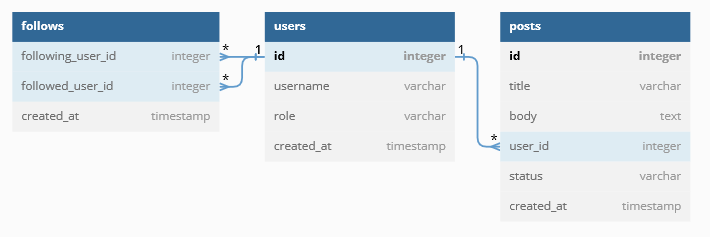
\includegraphics[width=\textwidth]{dbdiagram}
	\caption{Sample database visualising from: \cite{dbdiagram}}
	\label{fig:dbdiagram}
\end{figure}

\subsection{Suggestion of Structure Faults}

After the SQL has been parsed and the database has been displayed to the user, the application should provide advice and possible faults of the database, if there are any. This should be clear and direct, and it also should provide feedback as to how to fix this issue. This would involve an analysis of the database structure to see if there are any keys missing or an incorrect design of the database.

\subsection{Scope}
\label{subsec:scope}

A possible goal for this project was to create parsing for the DQL (Data Query Language). This would involve allowing the user to not only input their table structure but also their entries in the tables. This would allow the user to enter a query for the database, and this project would be able to parse the query and return the result of the query to the user. The user would then test for themselves to see if the returned entries were what they expected from their queries. 

However, this proved to be an additional feature that was not needed for the scope of this project. This application focuses on identifying database design flaws, parsing of queries could be a feature that could be added in future works of this project.

Another goal for this project was to create an algorithm to fix the issues that were detected in the database. Since the parsing has detected the errors, it would be possible to create a function to fix a problem for each kind of error. 

This could be done for creating keys and joining tables by foreign keys, however since it would be difficult to identify the context of the real world entities behind the database it would make it hard to automatically find the correct tables to link together by a foreign key. This would also not be very educational for the learners since this is not teaching the ways to correct the errors, it instead repairs the flaws for the learner not leaving much room for learning. 

\section{Requirements}

\begin{center}
	\captionof{table}{\label{fig:fr}Functional Requirement Table.}
	\setlength\extrarowheight{2pt}
	\begin{tabularx}{\textwidth}{|X|X|X|}
		
		\hline
		\textbf{Functional Requirement Number} & \textbf{Functional Requirement Name} & \textbf{Functional Requirement Description} \\
		\hline
		FR-1 & Enter SQL into website form. & The user can enter their SQL into the website form. \\
		\hline
		FR-1.1 & Enter SQL into the text area. & The user can paste the SQL code into the text area in the website. \\
		\hline
		FR-1.2 & Upload SQL file to website form. & The user can upload their SQL file to the website form. \\
		\hline
		FR-2 & Validate entered SQL. & If the SQL syntax is not valid then the user should be informed with the syntax error. \\
		\hline
		FR-3 & Visualise entered database. & If the SQL syntax is correct then the user should be able to visualise the entered database. \\
		\hline
		FR-4 & View highlighted syntax after visualising. & Once the database has been visualised, the user can switch to "syntax view" and be presented with highlighted syntax of the entered SQL. \\
		\hline
		FR-5 & The user can filter through data types of columns in syntax view. & Also in the syntax view the user can select data types to be highlighted to a different colour to make it easier to view them. \\
		\hline
		FR-6 & The user can view the flaws of the database. & The user can switch to the "Problem View" and view the list of flaws of the database if there are any. \\
		\hline
		FR-7 & The user can view the advice on how to fix the flaws identified. & The user can switch to the "Problem View" and view the feedback on how to fix the flaw for each of the issues. \\
		\hline
	\end{tabularx}
\end{center}

\newpage

\section{Process}
\label{sec:process}

For this project, a process adapted from Scrumban was used. The elements of Scrum that were incorporated were:  
\begin{itemize}
	\item Week-long sprints with weekly review and retrospective sessions for iterative planning at regular intervals.
	\item These meetings dictated how much work was pulled into the sprint based on complexity and priority of the work.
	\item Assured necessary levels of analysis and design before starting development.
\end{itemize}
The elements of Kanban that were incorporated were:
\begin{itemize}
	\item In addition to the weekly review and retrospective sessions, a short time was dedicated to process improvement.
	\item Kanban board to provide visualisation of the current items that were in progress, To-Do or in the Sprint Backlog.
	
	\begin{figure}[h!]
		\centering
		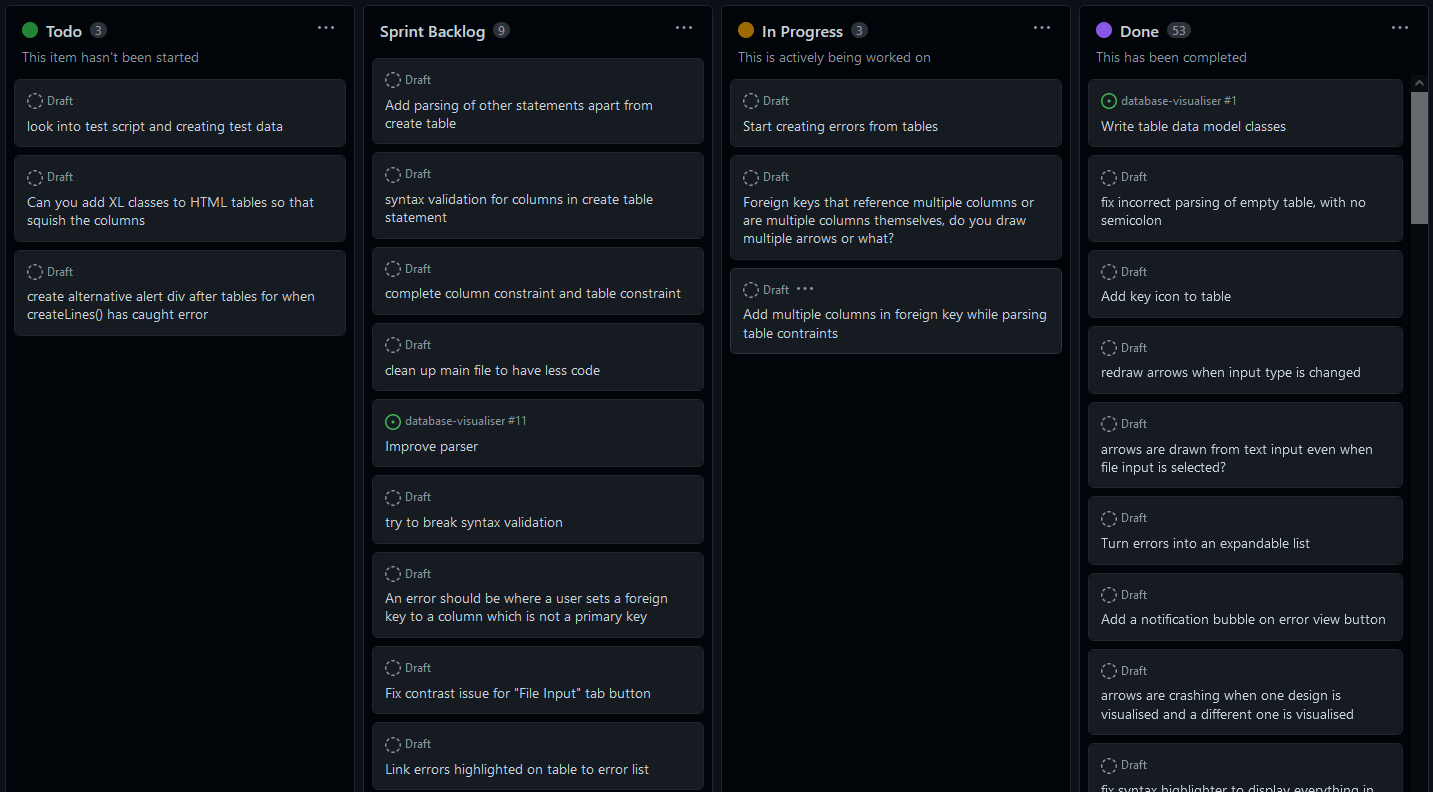
\includegraphics[width=\textwidth]{kanban}
		\caption{Kanban board used for the process of the project.}
		\label{fig:kanban}
	\end{figure}
\end{itemize}
